%!TeX root=../tese.tex
%("dica" para o editor de texto: este arquivo é parte de um documento maior)
% para saber mais: https://tex.stackexchange.com/q/78101

\chapter{Introduction}
\label{chap:intro}



What is the difference between computer science and software engineering? Both deal with computers, right? Are they not the same thing?

Computer science is the field focused on the theoretical powers of computers and the algorithms we write for them. Is this problem decidable? NP-complete? Can this thing be considered a Turing machine? Is P=NP? What functions can be approximated by neural networks? How can we color, with the minimal number of colors,  the vertices of a graph so that no two adjacent vertices have the same color? There are a myriad of important and interesting questions posed in this large field of study, but they are all centered around the computers and the theoretical.

This is where the computer science and software engineering fields differentiate themselves. Whereas one field is centered around computers and algorithms, the other is centered around the humans using these computers and implementing those algorithms, or to be more precise the relation and interactions between programmers and their code.

Software engineering is the field concerned with more mundane and practical aspects of programming, when we speak of code complexity we are talking about a more abstract concept than the well defined time complexity so ubiquitous in computer science theory, we are talking about the \textit{perceived} complexity of a program\footnote{This is not to say that software engineers have no interest in or knowledge of the theoretical aspects of computer science or that the two fields are completely disjoint, the best developers would take into account both the code's time complexity and its perceived complexity when writing a program.}. How easy is it to maintain? Is it readable? Can we easily test it for limit cases where bugs may be hiding? Is there code duplication that could be simplified?


Software engineering is the field of study concerned with the efficiency of the programmers and their code, not simply their code. How can we decrease the implementation time of a new feature and make developers more efficient? What are the bottlenecks in development? How do the developers organize themselves? What if they are part of a team? What about their code base? How do we measure the quality of a piece of code in regards to the value it brings to our clients or even to our own developers?

When trying to add a new feature to an existing software, a common first step is the re-writting of existing code, not the creation of new code as one might expect \citep{martinfowler}. The field of software engineering has a special name for this re-writting step, it is called \textit{refactoring}. To refactor a piece of code is to make simple and incremental changes in order to make it easier to work with and to be expanded upon. A survey from \citet{1001} shows that refactorings are a key element in the software development cycle. As can be seen in Figs.~\ref{fig:pizzas}, nearly four out of five developers in the 1,183 developers surveyed indicated that they refactored code every week or even almost every day. Two-thirds of these respondents said that they had refactoring sessions of an hour or longer during this time.



\begin{figure}
\centering
\begin{subfigure}{.5\textwidth}
  \centering
  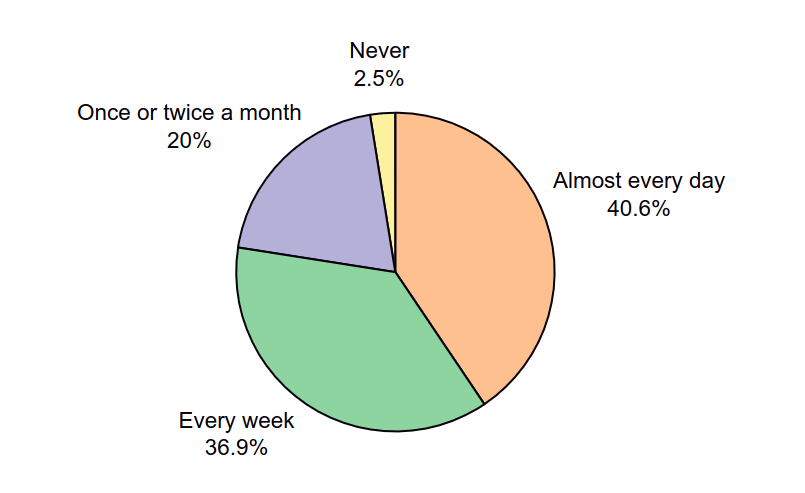
\includegraphics[width=1.2\linewidth]{figuras/q1pizza.png}
  \caption{In the past month, how
often have you performed any code refactoring? (Out of 1,181
respondents)}
  \label{fig:q1}
\end{subfigure}
\begin{subfigure}{.5\textwidth}
  \centering
  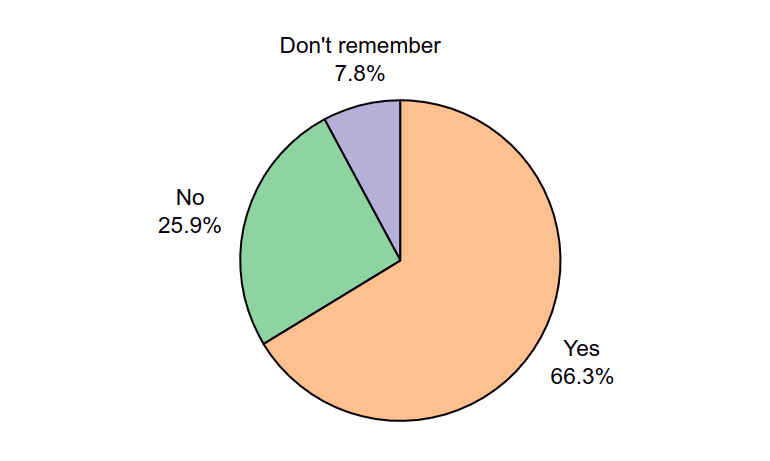
\includegraphics[width=1.2\linewidth]{figuras/q2pizza.png}
  \caption{During this time, did you ever refactor code for an hour or more in a single session? (Out of 1,145 respondents)}
  \label{fig:q2}
\end{subfigure}
\caption{Pie graphs of two of the 20 questions about refactoring answered by a group of 1,183 developers that were paying subscribers of IntelliJ Platform based IDEs. \citep{1001}}
\label{fig:pizzas}
\end{figure}


As one might expect from such an integral part of the software development cycle, extensive work \citep{1001, 7vista, abid202030} has been done to better understand how and when refactorings are done, or how to optimize and automate this often manual and repetitive task.
However, much of the work done is in order to automate a refactoring after a developer detected an opportunity and it is mediated by said developer. Let's say we want to break a long function into smaller functions, the developer has to go to the function and select the line span that they wish to extract.
The onus of refactoring the code is still on the developer, it is certainly faster than doing it manually without the help of these small automations but there is still room for improvement. Taking the same example as before, it would be even better if the IDE could suggest to the programmer which functions could use a refactoring or even which lines should be extracted. We posit that by making the refactoring process more automated and less reliant on the developer, refactoring would become even more commonplace and make developers in general more productive.

But how exactly could we achieve such automation? That is what we hope to answer in detail in the following chapters of this thesis dissertation. We intend to leverage the \textit{naturalness} of programming languages to train a machine learning model based on existing natural language processing techniques to automate refactorings of the function extraction type.


One might ask what is the ``naturalness of a programming language'' and why should we use NLP techniques in languages that are, by their very definition, non-natural but first we need to address what even is a natural language. 

The concept of natural language could be defined by what they are not: they are not artificially constructed and they are not ``rigid''. Let us take \citet{lang_file} definition of natural languages:


\begin{myquote}   
\textit{All languages exhibit all nine design features} \textbf{{\small
[as defined by \citet{hockett1960origin}:
Mode of Communication, Semanticity, Pragmatic Function, Interchangeability, Cultural Transmission, Arbitrariness, Discreteness, Displacement, Productivity]
}
} \textit{any communication system that does not is therefore not a language. Furthermore, as far as we know, only human communication
systems display all nine design features.} \textbf{[...]}

\qquad \textit{Because all languages exhibit the nine design features, does this mean that any communication system that exhibits all nine features should be considered a language? 
For example, there are formal languages, such as the formal logic used to write mathematical proofs and various computer languages. While these formal languages display all of the design features, they nevertheless differ in critical ways from languages such as English, Spanish, Mandarin, and Apache. For example, no child could ever acquire a computer language like C++ as his native language! 
Furthermore, a number of people engage in constructing languages that imitate human language as a hobby. There are many reasons that people might choose to do this. For example, the created language could be used in some sort of fictional universe, such as Klingon in the television series Star Trek or Dothraki and Valyrian in the series Game of Thrones. Or it might be designed to facilitate international communication, which was the goal of the designers of the language Esperanto. Other people, such as J.R.R. Tolkien, have constructed artificial languages just for fun.}
\par
\qquad \textit{Do we want to make a distinction between languages such as English, Spanish, Mandarin, and Apache, on the one hand, and Esperanto, Elvish, Dothraki, Valyrian, and Klingon, on the other? And how should we classify `formal' languages?
Although many of these questions are still open to debate and research, we will make the following distinctions }
\textbf{[...]}
\textit{we call natural languages, those languages that have evolved naturally in a speech community. The lexicon and grammar of a natural language have developed through generations of native speakers of that language. A constructed language, on the other hand, is one that has been specifically invented by a human and that may or may not imitate all the properties of a natural language.} \\\citet{lang_file}
\end{myquote}


Essentially, natural languages are languages that changed and evolved naturally alongside humans and are used for communication. That is not to say that a constructed language cannot become a natural language, an example is Modern Hebrew which was reconstructed and expanded from Ancient Hebrew (a liturgical and dead language) and then adopted by a particular community\footnote{The matter of Modern Hebrew's ``creation'', ``revival'' or ``(Re)vernacularization''\citep{spolsky1995conditions} and its characterization as a constructed language is a point of contention, this discussion is out of the scope of this work but we refer readers interested in a primer on the subject to \citet{izre2003emergence}.}.
We used non rigid to describe natural languages because of this capacity to change and evolve as well as its semantical robustness, even if a text contains a few mistakes its meaning may still be grasped while programming languages are brittle to mistakes (e.g. typos in variable names or parameter order inversion can drastically change the meaning of code or even break it).

\citet{lang_file} also brings us a sort of definition for formal languages:

\begin{myquote}
\textit{The distinction between constructed languages and formal languages is that formal languages are not the sort of system that a child can acquire naturally.} \\\citet{lang_file}
\end{myquote}


Although this is not wrong, most computer scientists would find it lacking as a definition. A more common formulation would be to define it as the set of all strings that can be derived from a formal grammar. That is to say, a formal language is defined (or generated) by its grammar and a piece of text can be identified as part of a formal language if it can be ``recognized'' by its grammar (i.e. parsed). More formally, a generative grammar is defined by a 4-tuple $(N, \Sigma, P, S)$ where $N$ is the set of non-terminal symbols, $\Sigma$ the set of terminal symbols (disjoint of $N$), $P$ the set of production or generation rules and $S$ the sentence or start symbol.

Table~\ref{table:grammar} depicts an example of the production rules part of a formal grammar for syntactically correct infix algebraic expressions for three variables, namely x, y and z, and depicts Fig~\ref{fig:parsetree} an example of a parse tree generated with these production rules for the expression $(x + y) \times x - z \times y / (x + x)$.


\begin{figure}[!ht]
\centerline{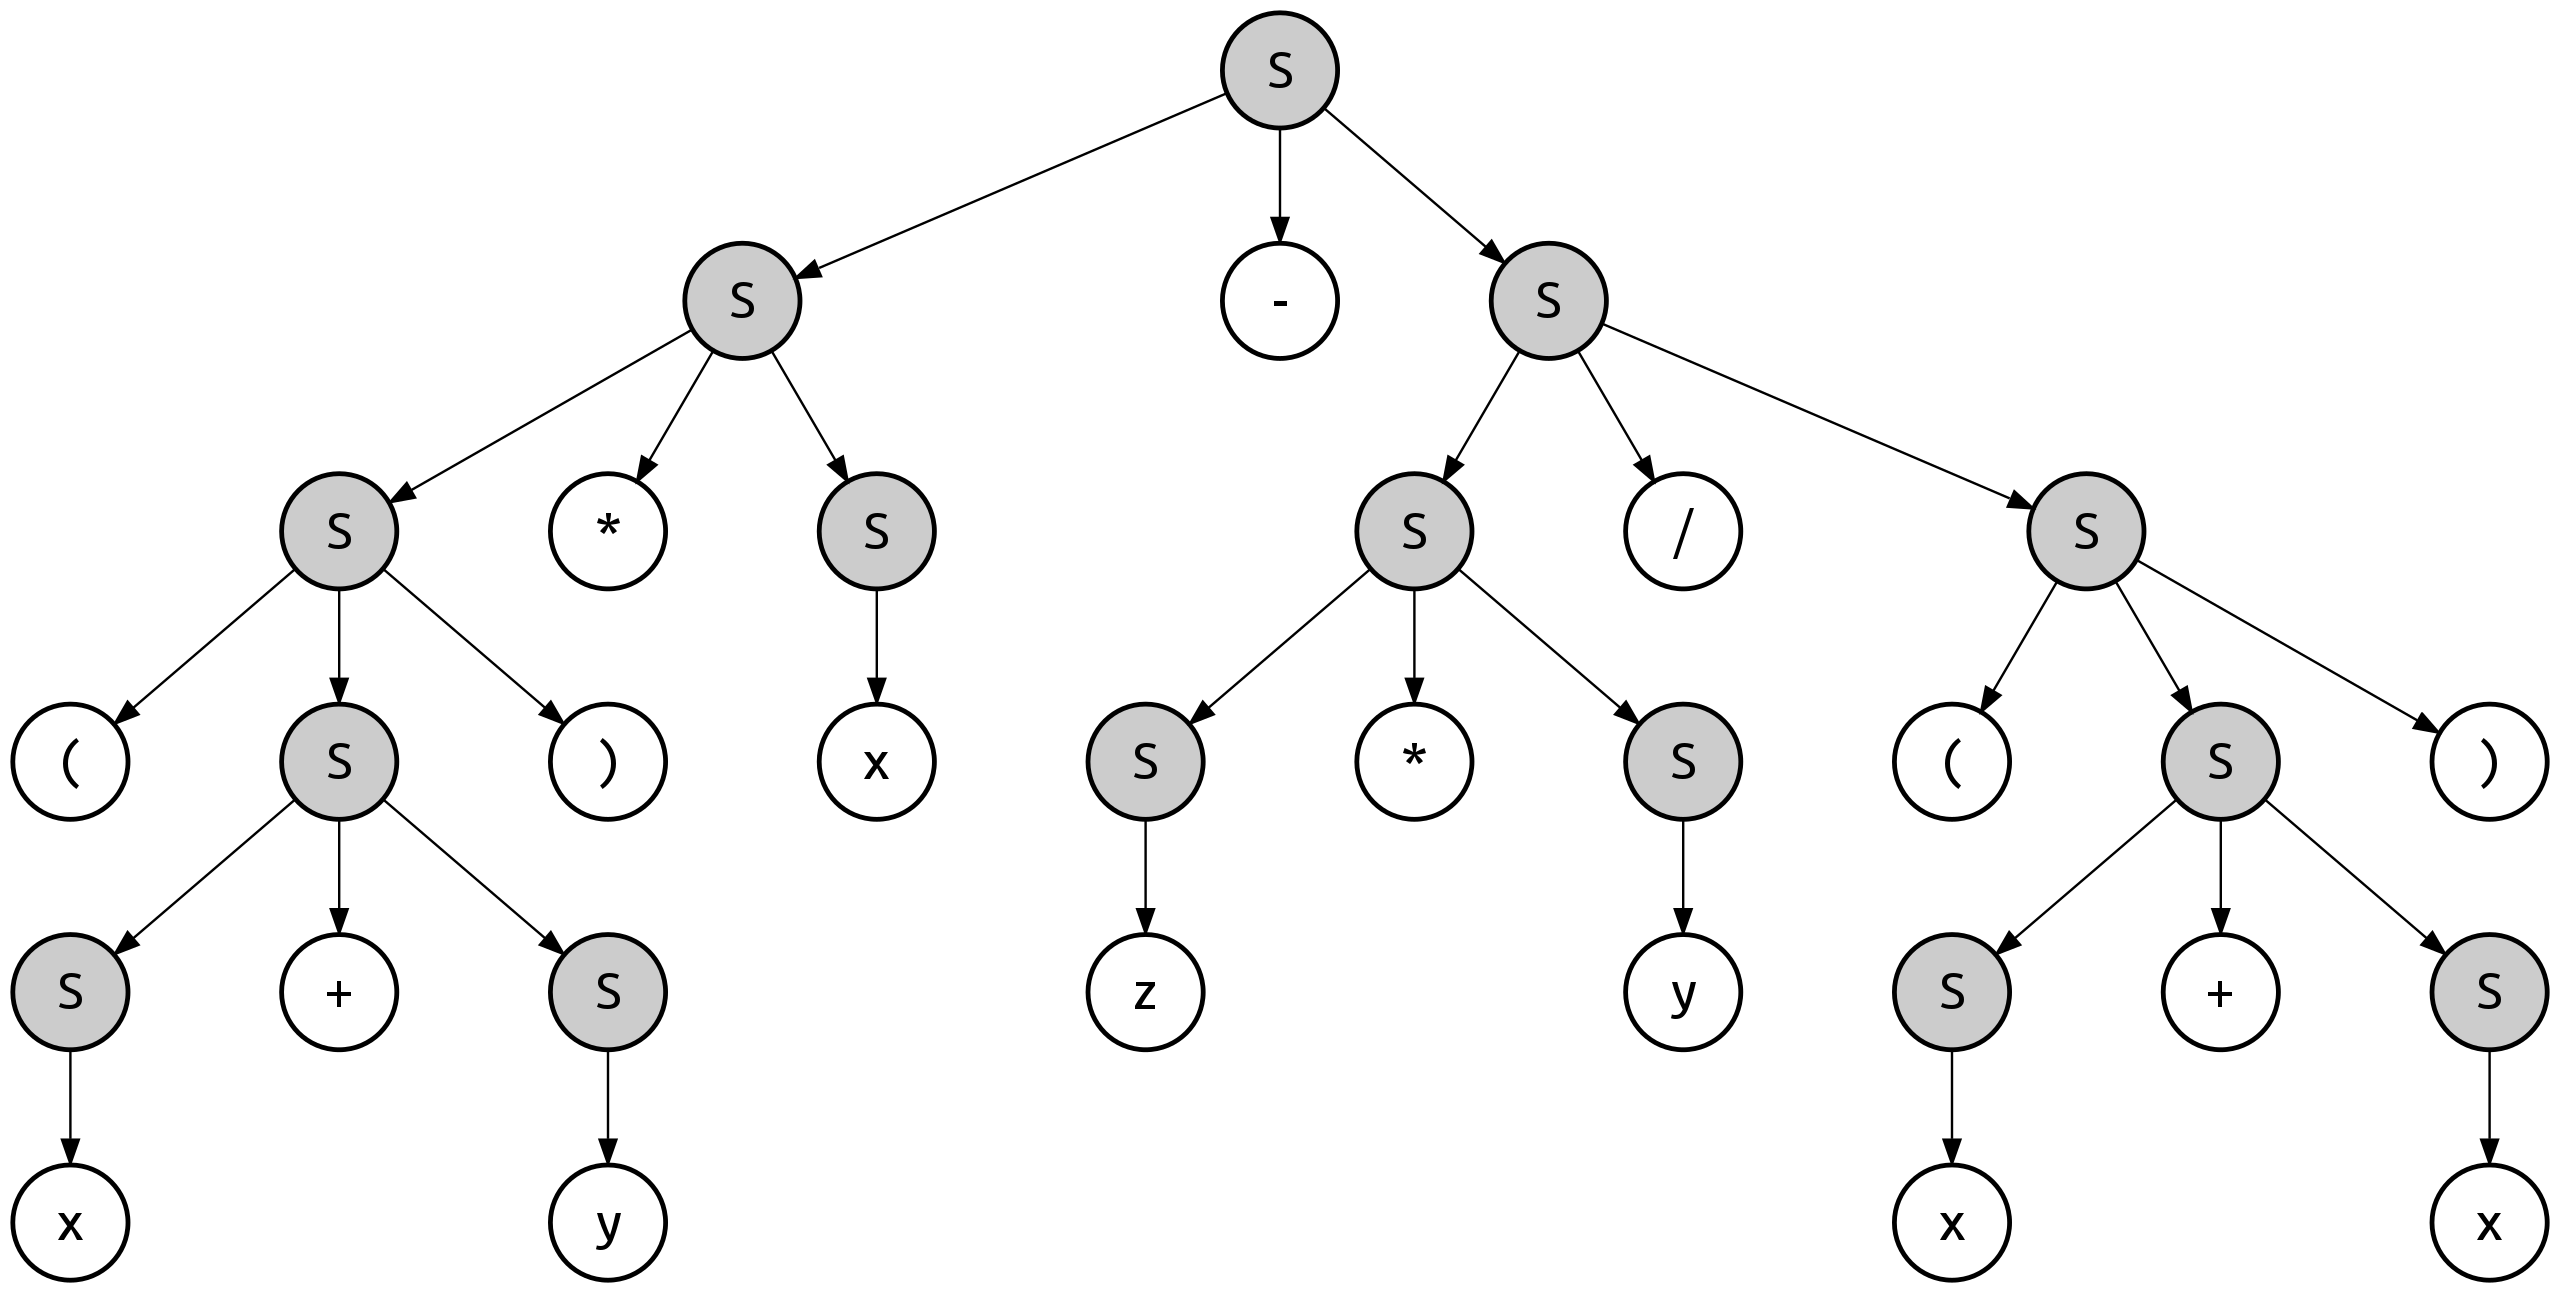
\includegraphics[width=\textwidth]{figuras/parse_tree_grammar.png}   }
\caption{One of the possible parse trees for the expression $(x + y) \times x - z \times y / (x + x)$ created from the production rules in Table~\ref{table:grammar}. Image from \citet{parse_tree}.}
\label{fig:parsetree}
\end{figure}

\begin{table}[]
\begin{tabular}{llll}
$S \rightarrow x$   &&& $S \rightarrow S + S$      \\
$S \rightarrow y$   &&& $S \rightarrow S - S$      \\
$S \rightarrow z$   &&& $S \rightarrow S \times S$ \\
$S \rightarrow (S)$ &&& $S \rightarrow S / S$     
\end{tabular}
\caption{Production rules of a formal grammar for syntactically correct infix algebraic expressions for three variables, namely x, y and z. In essence, the grammar is defined by these 8 production rules forming the $P$ set, $\{x, y, z, +, -, (, ), \times, /\}$ as the terminal symbols set $\Sigma$, $\{S\}$ as the set of non-terminal symbols $N$ and $S$ as the start symbol. Note that this grammar is ambiguous so it has multiple possible parse trees. }
\label{table:grammar}
\end{table}


Formal languages, such as programming languages, can still change and evolve, however this happens as punctuated changes (e.g. the release of Python 3 to substitute Python 2 and the sub-sequential break of compatibility) and in contrast to natural languages that work in a bottom up fashion through social dynamics \citep{croft2008evolutionary}, programming languages are designed top-down by a few designers for many users.

These are not their only differences, another example is that it is not clear if it is feasible to create a translation between natural languages such that the meaning is completely preserved\footnote{And also highly dependent on the definition of \textit{meaning} being used.}. However every mainstream\footnote{There are programming languages that are not developed with universal computation in mind, such as the BlooP \citep{bloop} and Charity \citep{charity} languages, however they are not widely adopted in the industry nor posses a sizable user base.} programming language is Turing complete \citep{turing} so it is always possible\footnote{Anyone who has worked in code translation may tell you that this can be ``easier said than done''. Code portability can be a challenging subject even if we ignore unusual Turing complete languages such as Microsoft's PowerPoint \citep{ppt}.} to exactly translate a piece of code from one language to another.

Nevertheless machine translation between natural languages is an ever thriving research topic. Furthermore, in recent years the area of NLP has seen explosive growth together with new neural network architectures (GRU \citep{GRU}, Transformers \citep{attention_is_all_you_need}, ELMo \citep{ELMo}, BERT \citep{BERT} to name only a few recent ones) and a skyrocketing success reaching even mainstream popularity through large language models such as GPT-4 \citep{gpt4} and LLaMA \citep{llama}. On the other hand, the use and success of machine learning models for analogous tasks in programming languages (e.g. translation between programming languages or transpilation) has been comparatively moderate so far.



Despite having several differences, natural and programming languages also share a series of particularly interesting commonalities that allow the application of models and techniques originally devised for NLP tasks into analogous programming language processing tasks.






This idea is succinctly defined in the naturalness hypothesis:


\begin{myquote}
\textbf{Naturalness Hypothesis. }
\textit{
Software is a form of human communication; software corpora have similar statistical properties to natural language corpora; and these properties can be exploited to build better software engineering tools.}  \\\citet{allamanis2018survey}
\end{myquote}

This insight that programming may be seen as a form of human communication is not by any means new and can be traced back to Donald E. Knuth concept of \textit{literate programming} from his titular work Literate Programming:

\begin{myquote}
\textit{I believe that the time is ripe
for significantly better documentation of programs, and
that we can best achieve this by considering programs
to be works of literature. Hence, my title: `Literate
Programming.'}
\\
\\
\qquad\textit{ Let us change our traditional attitude to the construction of programs: Instead of imagining that our
main task is to instruct a computer what to do, let us
concentrate rather on explaining to human beings what
we want a computer to do.}
\\
\\
\qquad \textit{The practitioner of literate programming can be regarded as an essayist, whose main concern is with exposition and excellence of style. Such an author, with
thesaurus in hand, chooses the names of variables carefully and explains what each variable means. He or she strives for a program that is comprehensible because its
concepts have been introduced in an order that is best
for human understanding, using a mixture of formal
and informal methods that re{\"i}nforce each other. }\\\citet{knuth1984literate}\end{myquote}


Although the naturalness hypothesis may not seem surprising to some, it is worth understanding the genesis of this naturalness. 

As stated by \citet{allamanis2018survey} ``\textit{naturalness of code seems to have a strong connection with the fact that developers prefer to write \citep{Allamanis_2014} and read \citep{7180076} code that is conventional, idiomatic, and familiar because it helps understanding and maintaining software systems}''.

This leads to the idea that code artifacts may contain recurring and predictable patterns that can be leveraged by machine learning models to perform a plethora of different tasks, in a not dissimilar way to how recurring and predictable patterns in linguistic corpora have been successfully utilized in NLP models.

\citet{naturalidade_original} demonstrated that corpus-based statistical language models can capture a high level of regularity in software, even more so than in english, and that this is not an artifact of the programming language syntax but rather it arises from the naturalness of the code.

They reason that, like natural languages, software is repetitive and predictable:

\begin{myquote}
    \textit{We begin with the conjecture that \emph{most software is also natural}, in the sense that it is created by humans at work, with all the attendant constraints and limitations} \textbf{[...]}
    \\
    \\
    \qquad \textit{Programming languages, in theory, are complex, flexible and powerful, but the programs that \underline{real} people \underline{actually} write are mostly simple and rather repetitive, and thus they have usefully predictable statistical properties that can be captured in \underline{statistical language models} and leveraged for software engineering tasks. }\\\citet{naturalidade_original} 
\end{myquote}

An important point raised was that \textbf{most} software is also natural, not all code ever written. One could easily argue that the hypothesis of human communication can be discarded when we are dealing with esoteric programming languages such as brainfuck \citep{brainfuck}, Piet \citep{piet} or Malbolge \citep{malbolge}, aptly named after the 8th circle of Hell from \citet{alighieri1788divina}. Fig.~\ref{fig:eso} presents three code snippets to help clarify how convoluted and deliberately obtuse esoteric languages can be designed to be. 
Being less extreme, not all code could be said to be ``readable'' or to be clearly and well structured, e.g. an inexperienced programmer's code\footnote{Recent evidence actually suggests that the amateur nature of inexperienced programmers may actually be beneficial for the corpus as was described in testimony given by Replit’s Head of AI in \citet{podcast_replit}, where they claim to have obtained a 50\% increase in performance when fine tuning their model on the replit codebase --- which contains a lot of code from people still in the process of learning how to program. However, our point stands that even if not all code could be considered natural it is likely relegated to a small part of softwares at large and would end up as an issue of data quality the same way data quality is an issue for NLP corpora.}, may not conform to best practices and contain confusing or out-write miss-leading function and variable names. If this is sufficient to classify the code as not natural is a matter out of the scope of this project, however we posit that those are rare instances in large successful projects that usually have naming conventions, contributing guidelines and code quality metrics and as such would not have a huge impact on data quality and training performance.

\begin{figure}[!ht]
\centerline{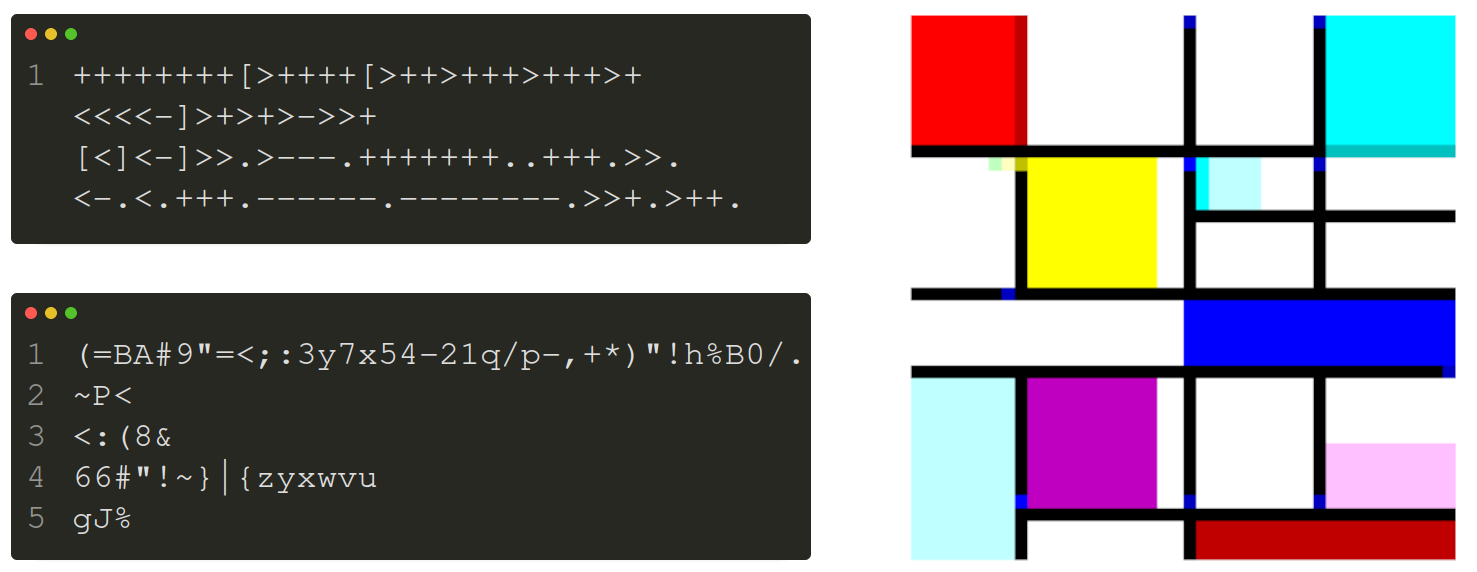
\includegraphics[width=\textwidth]{figuras/eso.png}   }
\caption{3 code snippets in esoteric languages. On the right the image that resembles a painting from Piet Mondrian is a program in the Piet language that prints the ``Piet'' string \citep{piet_image}. On the upper left is a ``Hello World!'' program written in brainfuck where only 8 characters (><+-.,[]) are available and each correspond to a different pointer operation \citep{brainfuck_codigo}. Lastly, on the lower left we have a \texttt{cat} program (that does not stop at EOF) written in Malbolge, a language designed to be as difficult to program in as possible with a ternary system, self-altering code and, once again, only 8 valid instructions \citep{malbolge_codigo}.}
\label{fig:eso}
\end{figure}



So far, this naturalness approach to programming languages has been shown to be fruitful many times. \citet{allamanis2018survey} make an extensive review of the literature compiling works that leverage in some way the ideas behind the naturalness hypothesis, there are too many to list here so we encourage interested readers to seek the original paper that is readily available online. Readers pressed for time may be interested in inspecting the tables since they compile most of the surveyed work in a systematic and well organized manner. It is important to note that this is not an exhaustive survey since it was published in 2018 and this field of study has by no means stopped since then. Two interesting and more recent works are the code2vec \citep{code2vec}, capable of abstracting the work done by a function by naming it based solely on information obtained through its abstract syntax tree and code2seq \citep{code2seq}, not only capable of predicting method names but also predicting natural language captions given partial and short code snippets, and to even generate method documentation.

We believe these ideas and the results we obtained during the course of this project serve as a proof of the soundness of our approach.


\section{Goals}

This project intends to accomplish two main goals:

\begin{itemize}
\item Understand if deep learning models are capable of predicting fine-grained refactorings, i.e. where exactly the source code should be refactored.
\item Create a model for automated function extraction.
\end{itemize}

\section{Organization}
The thesis is organized as follows: in Chapter~2 we define refactorings and propose a theoretical IDE plugin to better illustrate our objectives as well as provide some software engineering background; in
Chapter~3 we present the theoretical background of our models and other NLP and ML concepts; in Chapter~4 we present related work on automating refactorings; in Chapter~5 we explain how we built our dataset; in Chapter~6 we define the building blocks of our model followed by our experiments with those blocks in Chapter~7; and, finally, in Chapter~8 we give our concluding remarks and trace possible future steps.
